\documentclass[]{standalone}

\usepackage{../lenses}

\newcommand{\drawTwo}[5]{%x,y,align,v1,v2
  \draw(#1,#2) node[#3]{$v_{#4} + \overline{v_{#5}}$};
}
\newcommand{\drawThree}[6]{%x,%y,align,v1,v2,v3
  \draw(#1,#2) node[#3]{$v_{#4} + \overline{v_{#5}} + v_{#6}$};
}

\begin{document}
 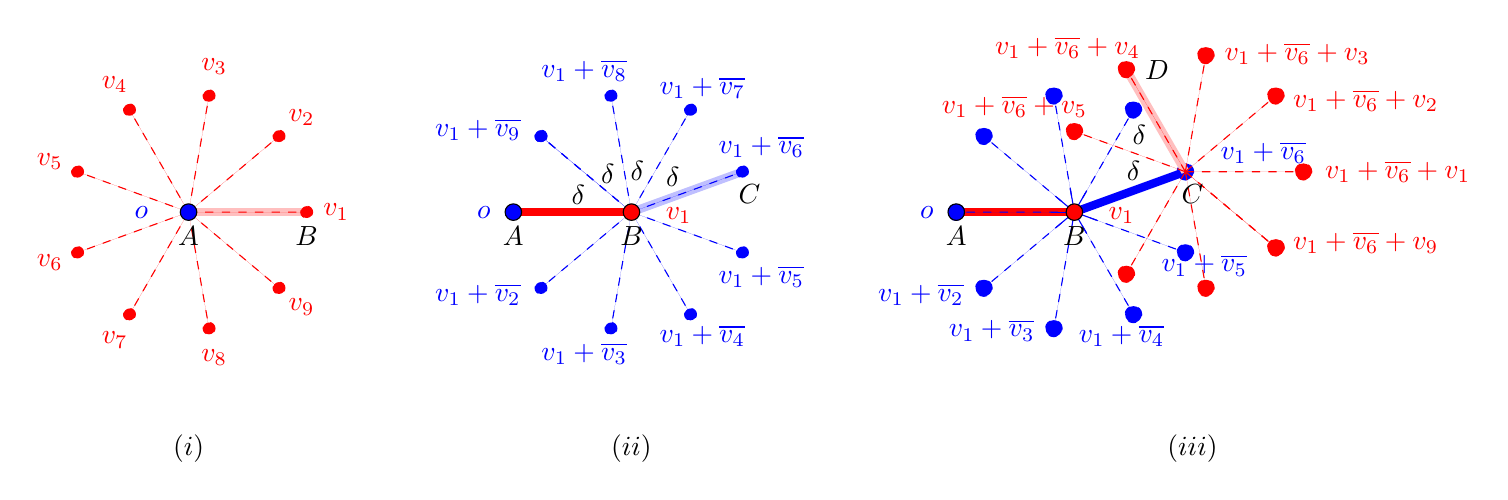
\begin{tikzpicture}
  \begin{scope}[scale=1.5]
  
   \begin{scope}[shift={(0,0)}]
    \draw[line width=3pt,red!25!white](0,0) -- (1,0);
    \foreach \x in {1,2,3,4,5,6,7,8,9} {
     \pgfmathsetmacro{\n}{40*(\x-1)}
     \draw[red,fill=red,dashed](0,0) -- (\n:1) circle(0.05)
      ++(\n:0.25) node{$v_\x$};
    }
    \draw[fill=blue](0,0) circle(0.07) ++(-0.4,+0.0) node[blue]{$o$};
    \draw(0,-0.2) node{$A$};
    \draw(1,-0.2) node{$B$};

    \path(0,-2) node{$(i)$};
   \end{scope}

   \begin{scope}[shift={(2.75,0)}]
   
    \draw[line width=3pt,red](0,0) -- (1,0);
    \begin{scope}[shift={(1,0)}]
     \draw[line width=3pt,blue!25!white](0,0) -- (20:1);
     \begin{scope}[blue]
      \foreach \x in {0,2,3,4,5,6,7,8,9} {
       \ifthenelse{\x=0}{ } {
        \pgfmathsetmacro{\n}{180+40*(\x-1)}
        \draw[fill=blue,dashed](0,0) -- (\n:1) circle(0.05);
       }
      }
      \drawTwo{+1.1}{+0.55}{}{1}{6}
      \drawTwo{+1.1}{-0.55}{}{1}{5}
      \drawTwo{+0.6}{+1.05}{}{1}{7}
      \drawTwo{+0.6}{-1.05}{}{1}{4}
      \drawTwo{-0.4}{+1.2 }{}{1}{8}
      \drawTwo{-0.4}{-1.2 }{}{1}{3}
      \drawTwo{-1.3}{+0.7 }{}{1}{9}
      \drawTwo{-1.3}{-0.7 }{}{1}{2}
     \end{scope}
    \end{scope}
    \draw[fill=blue](0,0) circle(0.07) ++(-0.25,+0.0) node[blue]{$o$};
    \draw[fill=red](0:1) circle(0.07) ++(+0.4,-0.03) node[red]{$v_1$};
    \draw(0,-0.2) node{$A$};
    \draw(1,-0.2) node{$B$};
    \draw(2,0.15) node{$C$};
    \draw(0.55,0.15) node{$\delta$};
    \draw(0.80,0.32) node{$\delta$};
    \draw(1.05,0.35) node{$\delta$};
    \draw(1.35,0.30) node{$\delta$};

    \path(1,-2) node{$(ii)$};
   \end{scope}

   \begin{scope}[shift={(6.5,0)}]

    \draw[line width=3pt,red](0,0) -- (1,0);

    \begin{scope}[shift={(0:1)}]
     \draw[line width=3pt,blue](0,0) -- (20:1);
     \begin{scope}[blue]
      \foreach \x [count=\c] in {0,2,3,4,5,6,0,0,0} {
       \pgfmathsetmacro{\n}{180+40*(\c-1)}
       \ifthenelse{\x=0}{ 
        \draw(0,0) -- (\n:0.2);
       } {
        \draw[fill=blue,dashed](0,0) -- (\n:1) circle(0.07);
       }
      }
      \drawTwo{+1.6}{+0.50}{}{1}{6}
      \drawTwo{+1.1}{-0.45}{}{1}{5}
      \drawTwo{+0.4}{-1.05}{}{1}{4}
      \drawTwo{-0.7}{-1.0 }{}{1}{3}
      \drawTwo{-1.3}{-0.7 }{}{1}{2}

      \begin{scope}[shift={(20:1)}]
       \begin{scope}[red]
        \draw[line width=3pt,red!25!white](0,0) -- (120:1);
        \foreach \x in {1,2,3,4,5,0,7,8,9} {
         \ifthenelse{\x=0}{ } {
          \pgfmathsetmacro{\m}{40*(\x-1)}
          \draw[fill=red,dashed](0,0) -- (\m:1) circle(0.07);
         }
        }
        \drawThree{+1.10}{+0.0 }{right}{1}{6}{1}
        \drawThree{+0.83}{+0.6 }{right}{1}{6}{2}
        \drawThree{+0.25}{+1.0 }{right}{1}{6}{3}
        \drawThree{-0.30}{+1.05}{left} {1}{6}{4}
        \drawThree{-0.75}{+0.55}{left} {1}{6}{5}
        \drawThree{+0.83}{-0.6 }{right}{1}{6}{9}
       \end{scope}
      \end{scope}

     \end{scope}
    \end{scope}
    \draw[fill=blue](0,0) circle(0.07) ++(-0.25,+0.0) node[blue]{$o$};
    \draw[fill=red](0:1) circle(0.07) ++(+0.4,-0.03) node[red]{$v_1$};
    \draw(+0.0,-0.20) node{$A$};
    \draw(+1.0,-0.20) node{$B$};
    \draw(+2.0,+0.15) node{$C$};
    \draw(+1.7,+1.20) node{$D$};
    \draw(1.50,0.35) node{$\delta$};
    \draw(1.55,0.65) node{$\delta$};
    

    \path(2,-2) node{$(iii)$};
   \end{scope}


  \end{scope}
 \end{tikzpicture}
\end{document}